\subsection{Ensayo con Carga}

Una vez realizado el ensayo sin carga, y verificado el funcionamiento sin fallas del puente de transistores, se puede proceder a la siguiente prueba. A diferencia del caso anterior, se va a ensayar el convertidor CC-CC completo, conectando el transformador y el inductor de salida $L_f$ a sus terminales correspondientes (ver figura \ref{test_setup}).\\

Como ya se mencionó, la fuente de laboratorio HP 6010A está encargada de proveer la corriente y tensión necesaria en el primario, mientras que la carga electrónica variable ITECH IT8514B+ se conecta en el terminal de salida del secundario y absorbe la corriente continua de la salida. La fuente se configuró en modo de tensión constante (operando a \SI[]{15}{\volt} o \SI[]{30}{\volt}) con limitador de corriente variable, y la carga electrónica en modo de resistencia constante.\\

En esta serie de ensayos se miden distintas variables representativas del sistema: tensión de salida $V_{out}$, tensión rectificada $V_{rect}$, corriente de salida $I_{out}$, corriente en el inductor $I_{Lf}$ y tensión del secundario $V_s$. Como en este caso va a existir circulación de corriente, incluso llegando a cargas cercanas a los \SI[]{100}{\watt} (un tercio de la máxima potencia del sistema), se va a poder observar como se comporta la plataforma frente a grandes circulaciones de corriente, incluido el funcionamiento del rectificador de diodos que no fue evaluado en las pruebas sin carga.\\

\subsubsection{Pruebas a 15 V}

Para proteger a los componentes, se comenzaron los ensayos con la fuente de laboratorio entregando una tensión continua de \SI[]{15}{\volt}, limitando la máxima tensión y corriente que cae sobre las llaves y diodos rectificadores.

\begin{figure}[h]
    \centering
    %\hspace{0.5em}
    \begin{subfigure}{0.48\textwidth}
        \centering
        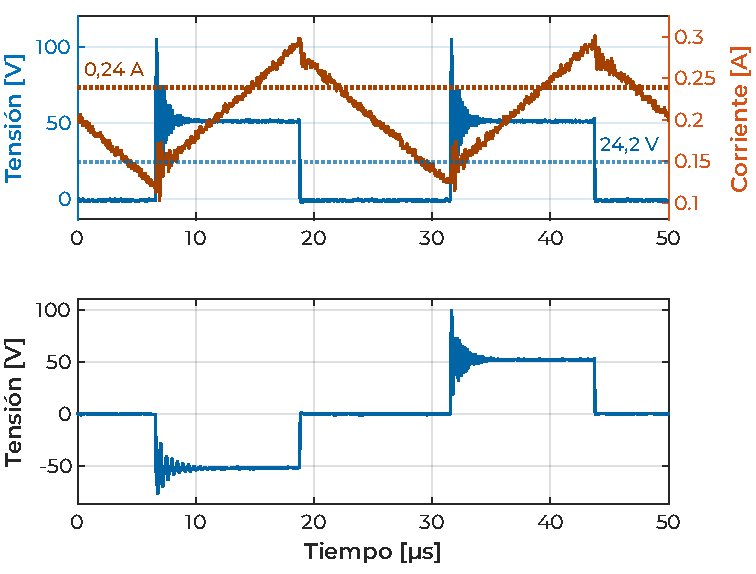
\includegraphics[width=\textwidth]{Imagenes/Con Carga - Caso 1.pdf}
        \caption{Ciclo de trabajo de 50\%.}
        \label{fig:ensayo_concarga15V_1}
    \end{subfigure}
    \hspace{0.5em}
    \begin{subfigure}{0.48\textwidth}
        \centering
        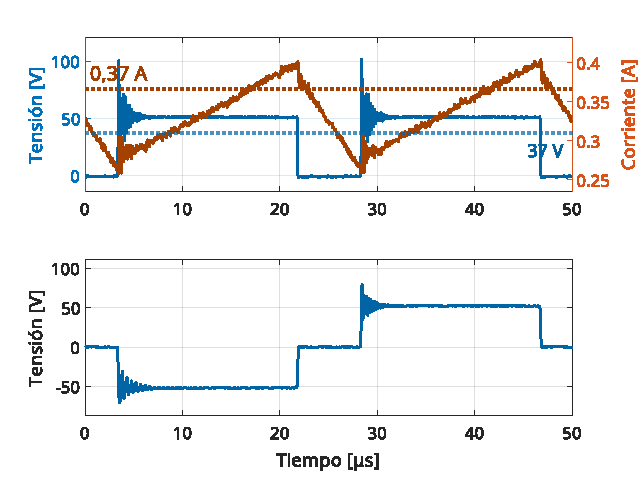
\includegraphics[width=\textwidth]{Imagenes/Con Carga - Caso 5.pdf}
        \caption{Ciclo de trabajo de 75\%.}
        \label{fig:ensayo_concarga15V_2}
    \end{subfigure}
    \caption{Tensión rectificada $V_{rect}$, corriente de inductor $I_{Lf}$ y tensión del bobinado secundario $V_{sec}$ para una carga de \SI[]{100}{\ohm} a la salida.}
    \label{fig:ensayo_concarga15V}
\end{figure}

\begin{figure}[h]
    \centering
    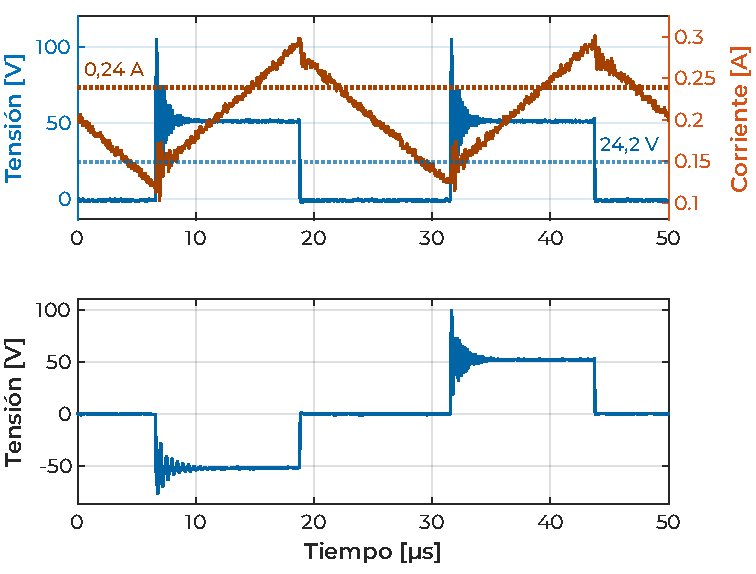
\includegraphics[scale=1]{Imagenes/Con Carga - Caso 1.pdf}
    \caption{Tensión rectificada $V_{rect}$ y corriente de inductor $I_{Lf}$ para una carga de \SI[]{100}{\ohm}, ciclo de trabajo de 50\% y tensión de entrada de \SI[]{15}{\volt}.}
    \label{ConCargaI}
\end{figure}

\lipsum[3]\\